\documentclass[../../../../main.tex]{subfiles}
\begin{document}

\begin{flushright}
\footnotesize\textit{【自動文字起こし・要確認】}
\end{flushright}

[解] 点$X$に対し, $\overrightarrow{OX} = \vec{x}$と定めると, $|\vec{a}_k| = \text{const} \ (k=1 \sim 6)$

\begin{center}
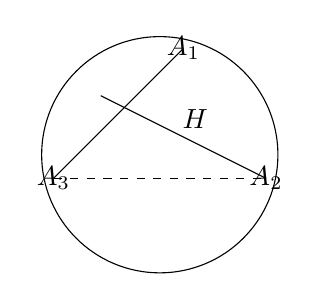
\begin{tikzpicture}[scale=1.5]
  \draw (0,0) circle (1);
  \node at (0.2, 0.9) {$A_1$};
  \node at (0.9, -0.2) {$A_2$};
  \node at (-0.9, -0.2) {$A_3$};
  \draw (0.2, 0.9) -- (-0.9, -0.2);
  \draw (0.9, -0.2) -- (-0.5, 0.5);
  \node at (0.3, 0.3) {$H$};
  \draw[dashed] (-0.9, -0.2) -- (0.9, -0.2);
\end{tikzpicture}
\end{center}

(i)
\begin{align*}
  &\overrightarrow{A_2H} \cdot \overrightarrow{A_1A_3} \\
  &= (\vec{a}_1+\vec{a}_3) \cdot (\vec{a}_3-\vec{a}_1) \\
  &= |\vec{a}_3|^2 - |\vec{a}_1|^2 = 0
\end{align*}
より $A_2H \perp A_1A_3$

同様にして, 各頂点と$H$を通る直線と, その対辺が直交するから$H$は垂心である 終

(ii) 選んだ3点$A_a, A_b, A_c$, のこりの3点$A_D, A_E, A_F$とする
(集合$\{A, B, \cdots, F\} = \{1, 2, 3, \cdots, 6\}$). (i)から$\triangle A_aA_bA_c$の垂心$H$は
\begin{equation}
  \vec{h} = \vec{a}_a + \vec{a}_b + \vec{a}_c \label{eq5_1}
\end{equation}
又, $\triangle A_DA_EA_F$の重心$G$として
\begin{equation}
  \vec{g} = \frac{1}{3} (\vec{a}_D + \vec{a}_E + \vec{a}_F) \label{eq5_2}
\end{equation}
\eqref{eq5_1}, \eqref{eq5_2}から$G, H$を通る直線上の点$X$は, $t \in \mathbb{R}$として
\[
  \vec{x} = \frac{1}{3} (\vec{a}_D + \vec{a}_E + \vec{a}_F) + \frac{t}{3} (3\vec{a}_a + 3\vec{a}_b + 3\vec{a}_c - \vec{a}_D - \vec{a}_E - \vec{a}_F)
\]
と表せる. $t = \frac{1}{4}$として
\[
  \vec{x} = \frac{1}{4} (\vec{a}_a + \cdots + \vec{a}_F) = \frac{1}{4} \sum_{k=1}^6 \vec{a}_k
\]
これは3点のえらび方によらないから, 題意は示された 終

\end{document}
